% Options for packages loaded elsewhere
\PassOptionsToPackage{unicode}{hyperref}
\PassOptionsToPackage{hyphens}{url}
%
\documentclass[
]{article}
\usepackage{amsmath,amssymb}
\usepackage{iftex}
\ifPDFTeX
  \usepackage[T1]{fontenc}
  \usepackage[utf8]{inputenc}
  \usepackage{textcomp} % provide euro and other symbols
\else % if luatex or xetex
  \usepackage{unicode-math} % this also loads fontspec
  \defaultfontfeatures{Scale=MatchLowercase}
  \defaultfontfeatures[\rmfamily]{Ligatures=TeX,Scale=1}
\fi
\usepackage{lmodern}
\ifPDFTeX\else
  % xetex/luatex font selection
\fi
% Use upquote if available, for straight quotes in verbatim environments
\IfFileExists{upquote.sty}{\usepackage{upquote}}{}
\IfFileExists{microtype.sty}{% use microtype if available
  \usepackage[]{microtype}
  \UseMicrotypeSet[protrusion]{basicmath} % disable protrusion for tt fonts
}{}
\makeatletter
\@ifundefined{KOMAClassName}{% if non-KOMA class
  \IfFileExists{parskip.sty}{%
    \usepackage{parskip}
  }{% else
    \setlength{\parindent}{0pt}
    \setlength{\parskip}{6pt plus 2pt minus 1pt}}
}{% if KOMA class
  \KOMAoptions{parskip=half}}
\makeatother
\usepackage{xcolor}
\usepackage[margin=1in]{geometry}
\usepackage{color}
\usepackage{fancyvrb}
\newcommand{\VerbBar}{|}
\newcommand{\VERB}{\Verb[commandchars=\\\{\}]}
\DefineVerbatimEnvironment{Highlighting}{Verbatim}{commandchars=\\\{\}}
% Add ',fontsize=\small' for more characters per line
\usepackage{framed}
\definecolor{shadecolor}{RGB}{248,248,248}
\newenvironment{Shaded}{\begin{snugshade}}{\end{snugshade}}
\newcommand{\AlertTok}[1]{\textcolor[rgb]{0.94,0.16,0.16}{#1}}
\newcommand{\AnnotationTok}[1]{\textcolor[rgb]{0.56,0.35,0.01}{\textbf{\textit{#1}}}}
\newcommand{\AttributeTok}[1]{\textcolor[rgb]{0.13,0.29,0.53}{#1}}
\newcommand{\BaseNTok}[1]{\textcolor[rgb]{0.00,0.00,0.81}{#1}}
\newcommand{\BuiltInTok}[1]{#1}
\newcommand{\CharTok}[1]{\textcolor[rgb]{0.31,0.60,0.02}{#1}}
\newcommand{\CommentTok}[1]{\textcolor[rgb]{0.56,0.35,0.01}{\textit{#1}}}
\newcommand{\CommentVarTok}[1]{\textcolor[rgb]{0.56,0.35,0.01}{\textbf{\textit{#1}}}}
\newcommand{\ConstantTok}[1]{\textcolor[rgb]{0.56,0.35,0.01}{#1}}
\newcommand{\ControlFlowTok}[1]{\textcolor[rgb]{0.13,0.29,0.53}{\textbf{#1}}}
\newcommand{\DataTypeTok}[1]{\textcolor[rgb]{0.13,0.29,0.53}{#1}}
\newcommand{\DecValTok}[1]{\textcolor[rgb]{0.00,0.00,0.81}{#1}}
\newcommand{\DocumentationTok}[1]{\textcolor[rgb]{0.56,0.35,0.01}{\textbf{\textit{#1}}}}
\newcommand{\ErrorTok}[1]{\textcolor[rgb]{0.64,0.00,0.00}{\textbf{#1}}}
\newcommand{\ExtensionTok}[1]{#1}
\newcommand{\FloatTok}[1]{\textcolor[rgb]{0.00,0.00,0.81}{#1}}
\newcommand{\FunctionTok}[1]{\textcolor[rgb]{0.13,0.29,0.53}{\textbf{#1}}}
\newcommand{\ImportTok}[1]{#1}
\newcommand{\InformationTok}[1]{\textcolor[rgb]{0.56,0.35,0.01}{\textbf{\textit{#1}}}}
\newcommand{\KeywordTok}[1]{\textcolor[rgb]{0.13,0.29,0.53}{\textbf{#1}}}
\newcommand{\NormalTok}[1]{#1}
\newcommand{\OperatorTok}[1]{\textcolor[rgb]{0.81,0.36,0.00}{\textbf{#1}}}
\newcommand{\OtherTok}[1]{\textcolor[rgb]{0.56,0.35,0.01}{#1}}
\newcommand{\PreprocessorTok}[1]{\textcolor[rgb]{0.56,0.35,0.01}{\textit{#1}}}
\newcommand{\RegionMarkerTok}[1]{#1}
\newcommand{\SpecialCharTok}[1]{\textcolor[rgb]{0.81,0.36,0.00}{\textbf{#1}}}
\newcommand{\SpecialStringTok}[1]{\textcolor[rgb]{0.31,0.60,0.02}{#1}}
\newcommand{\StringTok}[1]{\textcolor[rgb]{0.31,0.60,0.02}{#1}}
\newcommand{\VariableTok}[1]{\textcolor[rgb]{0.00,0.00,0.00}{#1}}
\newcommand{\VerbatimStringTok}[1]{\textcolor[rgb]{0.31,0.60,0.02}{#1}}
\newcommand{\WarningTok}[1]{\textcolor[rgb]{0.56,0.35,0.01}{\textbf{\textit{#1}}}}
\usepackage{longtable,booktabs,array}
\usepackage{calc} % for calculating minipage widths
% Correct order of tables after \paragraph or \subparagraph
\usepackage{etoolbox}
\makeatletter
\patchcmd\longtable{\par}{\if@noskipsec\mbox{}\fi\par}{}{}
\makeatother
% Allow footnotes in longtable head/foot
\IfFileExists{footnotehyper.sty}{\usepackage{footnotehyper}}{\usepackage{footnote}}
\makesavenoteenv{longtable}
\usepackage{graphicx}
\makeatletter
\def\maxwidth{\ifdim\Gin@nat@width>\linewidth\linewidth\else\Gin@nat@width\fi}
\def\maxheight{\ifdim\Gin@nat@height>\textheight\textheight\else\Gin@nat@height\fi}
\makeatother
% Scale images if necessary, so that they will not overflow the page
% margins by default, and it is still possible to overwrite the defaults
% using explicit options in \includegraphics[width, height, ...]{}
\setkeys{Gin}{width=\maxwidth,height=\maxheight,keepaspectratio}
% Set default figure placement to htbp
\makeatletter
\def\fps@figure{htbp}
\makeatother
\setlength{\emergencystretch}{3em} % prevent overfull lines
\providecommand{\tightlist}{%
  \setlength{\itemsep}{0pt}\setlength{\parskip}{0pt}}
\setcounter{secnumdepth}{5}
\ifLuaTeX
  \usepackage{selnolig}  % disable illegal ligatures
\fi
\usepackage{bookmark}
\IfFileExists{xurl.sty}{\usepackage{xurl}}{} % add URL line breaks if available
\urlstyle{same}
\hypersetup{
  pdftitle={Saving Outputs for Reproducible Research},
  pdfauthor={Gia-Huy Hoang},
  hidelinks,
  pdfcreator={LaTeX via pandoc}}

\title{Saving Outputs for Reproducible Research}
\author{Gia-Huy Hoang}
\date{2025-05-08}

\begin{document}
\maketitle

{
\setcounter{tocdepth}{2}
\tableofcontents
}
\subsection{Saving Output for Reproducible
Research}\label{saving-output-for-reproducible-research}

Saving output is a crucial part of responsible research data management
and directly supports the FAIR principles: making data Findable,
Accessible, Interoperable, and Reusable.

In this section, we will learn how to save cleaned datasets, update
metadata, export plots, and document our data processing in a
transparent and accessible way. These practices support reproducibility
and alignment with the FAIR principles.

\begin{Shaded}
\begin{Highlighting}[]
\FunctionTok{library}\NormalTok{(dplyr)}
\FunctionTok{library}\NormalTok{(readr)}
\end{Highlighting}
\end{Shaded}

\begin{center}\rule{0.5\linewidth}{0.5pt}\end{center}

\subsubsection{Saving Cleaned Datasets}\label{saving-cleaned-datasets}

For this section, you can continue from the previous section or load a
backup of the dataset from the \texttt{resources} folder:

\begin{Shaded}
\begin{Highlighting}[]
\NormalTok{Rdata\_path }\OtherTok{\textless{}{-}} \StringTok{"data/timeuse\_day3\_2.Rdata"}
\FunctionTok{load}\NormalTok{(Rdata\_path)}
\end{Highlighting}
\end{Shaded}

\paragraph{\texorpdfstring{Save Datasets as CSV or TSV for
\textbf{Interoperability} and
\textbf{Reusability}}{Save Datasets as CSV or TSV for Interoperability and Reusability}}\label{save-datasets-as-csv-or-tsv-for-interoperability-and-reusability}

Now, let's save this dataset into a CSV (Comma-Separated Values) or TSV
(Tab-Separated Values) file for sharing or reuse. Both are
\textbf{non-proprietary} formats that promote \textbf{interoperability}
and \textbf{accessibility}.

TSV is more versatile and enhances \textbf{reusability} due to:

\begin{itemize}
\tightlist
\item
  \textbf{CSV}: Uses commas to separate values, widely supported but may
  face issues if data contains commas.
\item
  \textbf{TSV}: Uses tabs as delimiters, avoiding comma-related problems
  and improving readability in text editors or spreadsheet software.
\end{itemize}

\begin{Shaded}
\begin{Highlighting}[]
\FunctionTok{write\_csv}\NormalTok{(js\_data, }\StringTok{"data/timeuse\_day4\_3\_20250502.csv"}\NormalTok{)}
\FunctionTok{write\_tsv}\NormalTok{(js\_data, }\StringTok{"data/timeuse\_day4\_3\_20250502.tsv"}\NormalTok{)}
\end{Highlighting}
\end{Shaded}

Both \texttt{write\_csv()} and \texttt{write\_tsv()} (from the
tidyverse) is a fast, UTF-8 CSV writer that by default skips row names
and matches \texttt{read\_csv()} (also a tidyverse function)
conventions, while base R's \texttt{write.csv()} is slower and writes a
row-names column unless you turn it off.

The \texttt{js\_data} object contains the dataset we used, transformed,
and modified up to now. In this session, we will assume this is our
final dataset to deposit into a repository such as OSF or Borealis.
Saving in \texttt{.csv} or \texttt{.tsv} makes sure our files are open
and usable across platforms, easily imported into other programming
languages, databases, or spreadsheet software.

\paragraph{Compression}\label{compression}

If you're working with large files, compressing your outputs (e.g., into
\texttt{.csv.gz}) helps conserve storage and facilitates faster file
transfers.

Why use \texttt{.gz} specifically? The \texttt{.gz} format is widely
supported, simple, and natively handled by R through the
\texttt{gzfile()} function. It's also compatible with most data
repositories and file-sharing platforms. Unlike \texttt{.zip}, which can
hold multiple files, \texttt{.gz} compresses a single file

\begin{Shaded}
\begin{Highlighting}[]
\NormalTok{con }\OtherTok{\textless{}{-}} \FunctionTok{gzfile}\NormalTok{(}\StringTok{"data/timeuse\_day4\_3\_20250502.gz"}\NormalTok{, }\StringTok{"wb"}\NormalTok{)}
\FunctionTok{write\_csv}\NormalTok{(js\_data, con)}
\end{Highlighting}
\end{Shaded}

\texttt{gzfile("…",\ "wb")} creates an R connection that writes directly
into a gzip-compressed file, and \texttt{write\_csv(js\_data,\ con)}
writes your data frame directly into that compressed CSV file.

Compression is especially helpful when sharing data through email or
uploading to repositories, enhancing \textbf{accessibility} by
minimizing bandwidth requirements. Even though in this example we're
working with a relatively small dataset, in real-world scenarios it's
common to encounter CSV files containing millions of rows---potentially
several gigabytes in size. In such cases, compression becomes not just
helpful but essential to efficiently store, transfer, and share data
files, especially when uploading to platforms like OSF or institutional
repositories.

\paragraph{Choosing Between Proprietary and Non-Proprietary
Formats}\label{choosing-between-proprietary-and-non-proprietary-formats}

Following the use of non-proprietary \texttt{.csv} and \texttt{.tsv}
formats for broad sharing, consider proprietary formats like
\texttt{.rds} or \texttt{.RData} only when your data is intended for use
within the sepecific ecosystem (in this case, it is R ecosystem).

\begin{itemize}
\tightlist
\item
  \textbf{Non-proprietary formats} (e.g., \texttt{.csv}, \texttt{.tsv}):
  Ensure \textbf{interoperability} across diverse systems and users, as
  discussed earlier, making data accessible to all.
\item
  \textbf{Proprietary formats} (e.g., \texttt{.rds}, \texttt{.RData}):
  Optimize \textbf{reusability} for R users by preserving R-specific
  data structures, but limit accessibility outside R.
\end{itemize}

In our dataset (\texttt{js\_data}), variables like \texttt{isFeelRushed}
(a binary factor: 1 = Yes, 0 = No) or other categorical variables (e.g.,
\texttt{popCenter}, or \texttt{feelRushed} might appear integer-like to
read\_csv(), which could misinterpret them as numeric integers instead
of factors. Saving as \texttt{.RData} preserves these R-specific data
types (e.g., factors, dates, or custom attributes), ensuring consistency
when the data is reloaded in R across different sections of our
analysis.

Here, we can save the \texttt{js\_data} in \texttt{.Rdata} format by
using the \texttt{save()} function:

\begin{Shaded}
\begin{Highlighting}[]
\FunctionTok{save}\NormalTok{(js\_data, }\AttributeTok{file =} \StringTok{"data/timeuse\_day4\_3.RData"}\NormalTok{)}
\end{Highlighting}
\end{Shaded}

\subsubsection{Updating and Saving Data
Dictionary}\label{updating-and-saving-data-dictionary}

To enhance \textbf{Findability} and \textbf{Reusability}, metadata must
be kept up to date. Metadata provides context about the data---what each
variable means, how values were coded, and how data were collected. This
makes it easier for others (including your future self!) to interpret
and reuse your data accurately.

One practical way to create and maintain metadata in R is to use a
\textbf{data dictionary}. A data dictionary is a structured summary that
describes each variable in a dataset, including its name, type, and
label or definition.

\paragraph{Types of Data Dictionaries: Human-Readable
vs.~Machine-Readable}\label{types-of-data-dictionaries-human-readable-vs.-machine-readable}

Data dictionaries can be designed as \textbf{human-readable} or
\textbf{machine-readable}, each serving distinct purposes with specific
advantages and limitations. Choosing the appropriate type depends on
your audience, whether it's researchers reading documentation or systems
processing metadata automatically.

\begin{itemize}
\tightlist
\item
  \textbf{Human-Readable Data Dictionary}:

  \begin{itemize}
  \tightlist
  \item
    \textbf{Description}: A human-readable data dictionary is formatted
    for easy comprehension by people, typically presented as a table in
    a spreadsheet (e.g., Excel) or document (e.g., PDF, Word). It
    includes plain-language descriptions in natural language (e.g.,
    English) and is designed to be intuitive for researchers, students,
    or non-technical collaborators. For example, a PDF document
    containing a table of variable descriptions is human-readable but
    often not machine-readable, as it lacks structured data that
    represents the relationships present in the dataset
  \item
    \textbf{Example} (PDF format):
    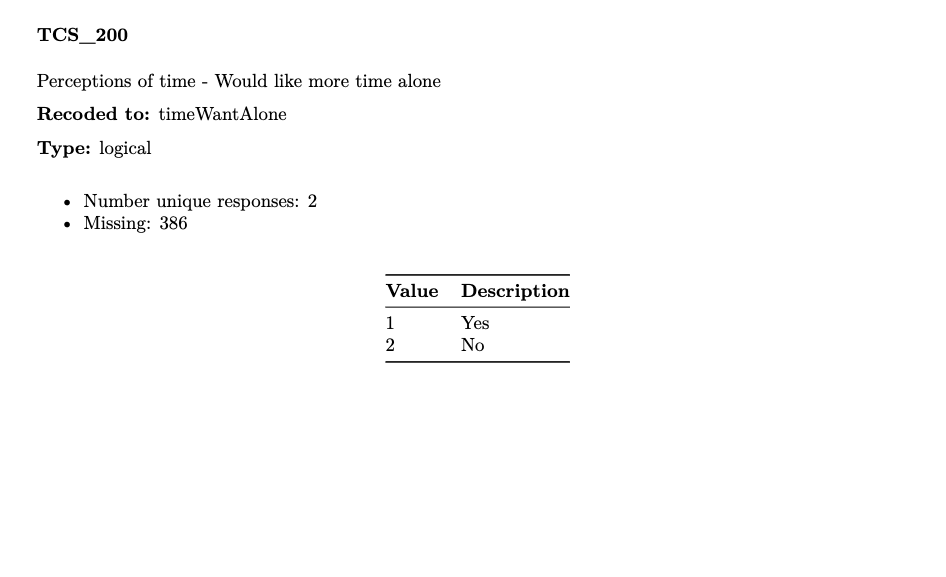
\includegraphics{images/4-ACT-3-datadictionaryPDF.png}
  \end{itemize}
\item
  \textbf{Machine-Readable Data Dictionary}:

  \begin{itemize}
  \tightlist
  \item
    \textbf{Description}: A machine-readable data dictionary uses
    structured formats like JSON, XML, YAML, or RDF, designed for
    software to parse and process automatically without human
    involvement. These formats align with metadata standards and are
    ideal for integration with data repositories or automated systems,
    enabling automatic data feeds and processing.
  \item
    \textbf{Example} (JSON format):
  \end{itemize}

\begin{Shaded}
\begin{Highlighting}[]
  \OtherTok{[}
  \FunctionTok{\{}
    \DataTypeTok{"variable"}\FunctionTok{:} \StringTok{"feelRushed"}\FunctionTok{,}
    \DataTypeTok{"type"}\FunctionTok{:} \StringTok{"integer"}\FunctionTok{,}
    \DataTypeTok{"description"}\FunctionTok{:} \StringTok{"Duration {-} Sleeping, resting, relaxing, sick in bed"}\FunctionTok{,}
    \DataTypeTok{"unique\_responses"}\FunctionTok{:} \DecValTok{274}\FunctionTok{,}
    \DataTypeTok{"missing"}\FunctionTok{:} \DecValTok{0}\FunctionTok{,}
    \DataTypeTok{"count"}\FunctionTok{:} \FloatTok{17390.0}\FunctionTok{,}
    \DataTypeTok{"mean"}\FunctionTok{:} \FloatTok{522.3948246118459}\FunctionTok{,}
    \DataTypeTok{"std"}\FunctionTok{:} \FloatTok{133.06481348435142}\FunctionTok{,}
    \DataTypeTok{"min"}\FunctionTok{:} \DecValTok{0}\ErrorTok{.}\DecValTok{0}\FunctionTok{,}
    \DataTypeTok{"percentile\_25"}\FunctionTok{:} \FloatTok{450.0}\FunctionTok{,}
    \DataTypeTok{"median"}\FunctionTok{:} \FloatTok{510.0}\FunctionTok{,}
    \DataTypeTok{"percentile\_75"}\FunctionTok{:} \FloatTok{585.0}\FunctionTok{,}
    \DataTypeTok{"max"}\FunctionTok{:} \FloatTok{1440.0}
  \FunctionTok{\}}\OtherTok{,}
  \FunctionTok{\{}
    \DataTypeTok{"variable"}\FunctionTok{:} \StringTok{"durSleep"}\FunctionTok{,}
    \DataTypeTok{"type"}\FunctionTok{:} \StringTok{"factor"}\FunctionTok{,}
    \DataTypeTok{"description"}\FunctionTok{:} \StringTok{"General time use {-} Feel rushed"}\FunctionTok{,}
    \DataTypeTok{"unique\_responses"}\FunctionTok{:} \DecValTok{6}\FunctionTok{,}
    \DataTypeTok{"missing"}\FunctionTok{:} \DecValTok{62}\FunctionTok{,}
    \DataTypeTok{"levels"}\FunctionTok{:} \OtherTok{[}
      \FunctionTok{\{}\DataTypeTok{"value"}\FunctionTok{:} \FloatTok{1.0}\FunctionTok{,} \DataTypeTok{"label"}\FunctionTok{:} \StringTok{"Every day"}\FunctionTok{\}}\OtherTok{,}
      \FunctionTok{\{}\DataTypeTok{"value"}\FunctionTok{:} \FloatTok{2.0}\FunctionTok{,} \DataTypeTok{"label"}\FunctionTok{:} \StringTok{"A few times a week"}\FunctionTok{\}}\OtherTok{,}
      \FunctionTok{\{}\DataTypeTok{"value"}\FunctionTok{:} \FloatTok{3.0}\FunctionTok{,} \DataTypeTok{"label"}\FunctionTok{:} \StringTok{"About once a week"}\FunctionTok{\}}\OtherTok{,}
      \FunctionTok{\{}\DataTypeTok{"value"}\FunctionTok{:} \FloatTok{4.0}\FunctionTok{,} \DataTypeTok{"label"}\FunctionTok{:} \StringTok{"About once a month"}\FunctionTok{\}}\OtherTok{,}
      \FunctionTok{\{}\DataTypeTok{"value"}\FunctionTok{:} \FloatTok{5.0}\FunctionTok{,} \DataTypeTok{"label"}\FunctionTok{:} \StringTok{"Less than once a month"}\FunctionTok{\}}
      \FunctionTok{\{}\DataTypeTok{"value"}\FunctionTok{:} \FloatTok{6.0}\FunctionTok{,} \DataTypeTok{"label"}\FunctionTok{:} \StringTok{"Never"}\FunctionTok{\}}      
    \OtherTok{]}
  \FunctionTok{\}}
\OtherTok{]}
\end{Highlighting}
\end{Shaded}

\begin{verbatim}
##   [
##   {
##     "variable": "feelRushed",
##     "type": "integer",
##     "description": "Duration - Sleeping, resting, relaxing, sick in bed",
##     "unique_responses": 274,
##     "missing": 0,
##     "count": 17390.0,
##     "mean": 522.3948246118459,
##     "std": 133.06481348435142,
##     "min": 0.0,
##     "percentile_25": 450.0,
##     "median": 510.0,
##     "percentile_75": 585.0,
##     "max": 1440.0
##   },
##   {
##     "variable": "durSleep",
##     "type": "factor",
##     "description": "General time use - Feel rushed",
##     "unique_responses": 6,
##     "missing": 62,
##     "levels": [
##       {"value": 1.0, "label": "Every day"},
##       {"value": 2.0, "label": "A few times a week"},
##       {"value": 3.0, "label": "About once a week"},
##       {"value": 4.0, "label": "About once a month"},
##       {"value": 5.0, "label": "Less than once a month"}
##       {"value": 6.0, "label": "Never"}      
##     ]
##   }
## ]
\end{verbatim}
\end{itemize}

\begin{longtable}[]{@{}
  >{\raggedright\arraybackslash}p{(\columnwidth - 4\tabcolsep) * \real{0.1412}}
  >{\raggedright\arraybackslash}p{(\columnwidth - 4\tabcolsep) * \real{0.4118}}
  >{\raggedright\arraybackslash}p{(\columnwidth - 4\tabcolsep) * \real{0.4471}}@{}}
\toprule\noalign{}
\begin{minipage}[b]{\linewidth}\raggedright
\textbf{Aspect}
\end{minipage} & \begin{minipage}[b]{\linewidth}\raggedright
\textbf{Human-Readable Data Dictionary}
\end{minipage} & \begin{minipage}[b]{\linewidth}\raggedright
\textbf{Machine-Readable Data Dictionary}
\end{minipage} \\
\midrule\noalign{}
\endhead
\bottomrule\noalign{}
\endlastfoot
\textbf{Pros} & \textbf{Accessibility}: Easy to read, supports
\textbf{reusability} for non-technical users. \textbf{Ease of Creation}:
Manual or CSV export, minimal tools needed.\textbf{Broad Usability}:
Suits workshops/reports, enhances \textbf{accessibility}. &
\textbf{Interoperability}: JSON/XML enable automation, repository
integration. \textbf{Efficiency}: Programmatic updates reduce errors for
large datasets. \textbf{Standardization}: Metadata standards enhance
\textbf{findability}. \\
\textbf{Cons} & \textbf{Limited Automation}: Unstructured, hard to
parse, hinders \textbf{interoperability}. \textbf{Manual Maintenance}:
Manual updates risk errors in large datasets. \textbf{Scalability
Issues}: Inefficient for many variables. \textbf{Non-FAIR Compliance}:
Lacks algorithmic processing, incompatible with FAIR. &
\textbf{Technical Barrier}: Needs scripting, challenging for users.
\textbf{Reduced Accessibility}: Complex without tools. \textbf{Format
Dependency}: JSON/XML may lack universal support. \textbf{Learning
Curve}: Structured formats hard for new users. \\
\end{longtable}

The human-readable PDF dictionary provided in the workshop is ideal for
learning and quick reference. For long-term storage or submission to
repositories like OSF or Borealis, convert it to a machine-readable
format to maximize \emph{Interoperability} and \emph{Findability}

\subsubsection{Documenting What Has Been
Changed}\label{documenting-what-has-been-changed}

Use your RMarkdown file as a living logbook. Write clear descriptions of
how your data has been transformed, which variables have been changed,
removed, or created. This documentation improves \textbf{transparency},
promotes \textbf{reusability}.

Example explanation:

\begin{quote}
``We filtered the dataset to include only respondents who feel rushed at
least once a week (\texttt{feelRushed} ≤ 3), and retained only time-use
columns for analysis.''
\end{quote}

Remember that we can create the \texttt{rushed} and \texttt{not\_rushed}
data frames by filtering \texttt{isFeelRushed\ ==\ 1} for rushed
participants and \texttt{isFeelRushed\ ==\ 0} for those who are not
rushed.

\begin{Shaded}
\begin{Highlighting}[]
\NormalTok{rushed }\OtherTok{\textless{}{-}}\NormalTok{ js\_data }\SpecialCharTok{|\textgreater{}} 
  \FunctionTok{filter}\NormalTok{(isFeelRushed }\SpecialCharTok{==} \DecValTok{1}\NormalTok{)}

\NormalTok{not\_rushed }\OtherTok{\textless{}{-}}\NormalTok{ js\_data }\SpecialCharTok{|\textgreater{}} 
  \FunctionTok{filter}\NormalTok{(isFeelRushed }\SpecialCharTok{==} \DecValTok{0}\NormalTok{)}
\end{Highlighting}
\end{Shaded}

And then, you can also track changes quantitatively:

\begin{Shaded}
\begin{Highlighting}[]
\NormalTok{summary\_changes }\OtherTok{\textless{}{-}} \FunctionTok{data.frame}\NormalTok{(}
  \AttributeTok{Step =} \FunctionTok{c}\NormalTok{(}\StringTok{"Original rows"}\NormalTok{, }\StringTok{"Filtered for isFeelRushed == 1"}\NormalTok{, }\StringTok{"Final rows"}\NormalTok{),}
  \AttributeTok{Count =} \FunctionTok{c}\NormalTok{(}\FunctionTok{nrow}\NormalTok{(js\_data), }\FunctionTok{sum}\NormalTok{(js\_data}\SpecialCharTok{$}\NormalTok{isFeelRushed }\SpecialCharTok{==} \DecValTok{1}\NormalTok{, }\AttributeTok{na.rm =} \ConstantTok{TRUE}\NormalTok{), }\FunctionTok{nrow}\NormalTok{(rushed))}
\NormalTok{)}
\NormalTok{summary\_changes}
\end{Highlighting}
\end{Shaded}

\begin{verbatim}
##                             Step Count
## 1                  Original rows 17390
## 2 Filtered for isFeelRushed == 1 12689
## 3                     Final rows 12689
\end{verbatim}

Such logs help other researchers understand your workflow and replicate
or build upon your analysis.

\subsubsection{Saving Plots}\label{saving-plots}

Exporting plots in multiple formats ensures your visualizations are
\textbf{reusable} and \textbf{accessible} for different purposes:
publication, presentation, or web display.

Let's first again generate the scatterplot to show the association
between sleep and work duration from previous section.

\begin{Shaded}
\begin{Highlighting}[]
\FunctionTok{library}\NormalTok{(ggplot2)}

\NormalTok{p }\OtherTok{\textless{}{-}} \FunctionTok{ggplot}\NormalTok{(js\_data, }\FunctionTok{aes}\NormalTok{(durWork, durSleep)) }\SpecialCharTok{+}
  \FunctionTok{geom\_point}\NormalTok{(}\AttributeTok{color =} \StringTok{"\#2D5E7F"}\NormalTok{, }\AttributeTok{alpha =}\NormalTok{ .}\DecValTok{2}\NormalTok{) }\SpecialCharTok{+}
  \FunctionTok{geom\_smooth}\NormalTok{(}\AttributeTok{method =}\NormalTok{ lm, }\AttributeTok{color =} \StringTok{"black"}\NormalTok{) }\SpecialCharTok{+}
  \FunctionTok{xlab}\NormalTok{(}\StringTok{"Minutes Spent Working"}\NormalTok{) }\SpecialCharTok{+}
  \FunctionTok{ylab}\NormalTok{ (}\StringTok{"Minutes Spent Sleeping"}\NormalTok{) }\SpecialCharTok{+}
  \FunctionTok{scale\_x\_continuous}\NormalTok{(}\AttributeTok{breaks =} \FunctionTok{seq}\NormalTok{(}\DecValTok{0}\NormalTok{, }\DecValTok{1500}\NormalTok{, }\DecValTok{250}\NormalTok{)) }\SpecialCharTok{+}
  \FunctionTok{labs}\NormalTok{(}\AttributeTok{title =} \StringTok{"Association Between Working and Sleeping"}\NormalTok{) }\SpecialCharTok{+}
  \FunctionTok{theme}\NormalTok{(}\AttributeTok{text =} \FunctionTok{element\_text}\NormalTok{(}\AttributeTok{size =} \DecValTok{18}\NormalTok{))}

\NormalTok{p}
\end{Highlighting}
\end{Shaded}


\includegraphics{4-ACT-3-SavingOutput_files/figure-latex/unnamed-chunk-8-1.pdf}

\paragraph{Save as PNG}\label{save-as-png}

\begin{Shaded}
\begin{Highlighting}[]
\FunctionTok{ggsave}\NormalTok{(}
  \AttributeTok{filename =} \StringTok{"outputs/association\_sleep\_working\_day4.png"}\NormalTok{, }
  \AttributeTok{plot =}\NormalTok{ p, }
  \AttributeTok{width =} \DecValTok{8}\NormalTok{, }
  \AttributeTok{height =} \DecValTok{6}\NormalTok{, }
  \AttributeTok{dpi =} \DecValTok{300}
\NormalTok{  )}
\end{Highlighting}
\end{Shaded}

\texttt{ggsave()} is a \texttt{ggplot2} function that saves your last
(or specified) plot to a file, automatically picking the correct format
from the filename extension and letting you set size and resolution.

This format is suitable for web use or slide presentations. PNG is a
raster format that offers high quality and is widely supported across
platforms.

\paragraph{Save as PDF}\label{save-as-pdf}

\begin{Shaded}
\begin{Highlighting}[]
\FunctionTok{ggsave}\NormalTok{(}
  \AttributeTok{filename =} \StringTok{"outputs/association\_sleep\_working\_day4.pdf"}\NormalTok{, }
  \AttributeTok{plot =}\NormalTok{ p, }
  \AttributeTok{width =} \DecValTok{8}\NormalTok{, }
  \AttributeTok{height =} \DecValTok{6}\NormalTok{)}
\end{Highlighting}
\end{Shaded}

PDF files preserve vector graphics, which means your plot can be resized
without losing quality. This is especially useful for embedding in
academic papers or generating printer-friendly outputs.

\paragraph{Save as TIFF (Use Cairo on
macOS)}\label{save-as-tiff-use-cairo-on-macos}

\begin{Shaded}
\begin{Highlighting}[]
\FunctionTok{ggsave}\NormalTok{(}
  \AttributeTok{filename =} \StringTok{"outputs/association\_sleep\_working\_day4.tiff"}\NormalTok{,}
  \AttributeTok{plot     =}\NormalTok{ p,}
  \AttributeTok{width    =} \DecValTok{8}\NormalTok{,}
  \AttributeTok{height   =} \DecValTok{6}\NormalTok{,}
  \AttributeTok{dpi      =} \DecValTok{600}\NormalTok{,}
  \AttributeTok{device   =} \StringTok{"tiff"}
\NormalTok{)}
\end{Highlighting}
\end{Shaded}

TIFF is often requested by academic journals for its high resolution.

Saving plots in appropriate formats facilitates sharing and integration
in different dissemination workflows.

\subsubsection{Exporting the Full Document as PDF or
HTML}\label{exporting-the-full-document-as-pdf-or-html}

Once you've saved individual datasets and plots, you'll often want to
bundle your \emph{entire} analysis---code, text, figures, and
tables---into a single file. You can export your RMarkdown document as a
\textbf{PDF} for a polished, human-readable output or as \textbf{HTML}
for a dynamic, web-friendly format. Each format has distinct advantages
and limitations, depending on your needs.

\begin{longtable}[]{@{}
  >{\raggedright\arraybackslash}p{(\columnwidth - 4\tabcolsep) * \real{0.2667}}
  >{\raggedright\arraybackslash}p{(\columnwidth - 4\tabcolsep) * \real{0.3556}}
  >{\raggedright\arraybackslash}p{(\columnwidth - 4\tabcolsep) * \real{0.3778}}@{}}
\toprule\noalign{}
\begin{minipage}[b]{\linewidth}\raggedright
\textbf{Aspect}
\end{minipage} & \begin{minipage}[b]{\linewidth}\raggedright
\textbf{PDF Output}
\end{minipage} & \begin{minipage}[b]{\linewidth}\raggedright
\textbf{HTML Output}
\end{minipage} \\
\midrule\noalign{}
\endhead
\bottomrule\noalign{}
\endlastfoot
\textbf{Pros} & - Human-readable.- Universally accessible.- Consistent
formatting.- Ideal for formal distribution (e.g., publications,
reports). & - Machine-readable.- Supports interactivity (e.g.,
collapsible code).- Web-friendly.- Smaller file sizes. \\
\textbf{Cons} & - Not machine-readable. - Lacks interactivity. - Large
file sizes.- Limited for web-based sharing. & - Requires web browser or
specific software.- Less consistent formatting across devices.- May need
technical setup for sharing. \\
\end{longtable}

In this section, we can practice to export our RMarkdown document as
either PDF or HTML.

\paragraph{1. Add (or confirm) your YAML
header}\label{add-or-confirm-your-yaml-header}

At the very top of your \texttt{.Rmd} file, ensure you have a YAML
header supporting both PDF and HTML outputs:

\begin{Shaded}
\begin{Highlighting}[]
\PreprocessorTok{{-}{-}{-}}
\FunctionTok{title}\KeywordTok{:}\AttributeTok{ }\StringTok{"RDM Jumpstart Workshop"}
\FunctionTok{author}\KeywordTok{:}\AttributeTok{ }\StringTok{"Your Name"}
\FunctionTok{date}\KeywordTok{:}\AttributeTok{ }\StringTok{"2025{-}05{-}08"}
\FunctionTok{output}\KeywordTok{:}
\AttributeTok{  }\FunctionTok{pdf\_document}\KeywordTok{:}
\AttributeTok{    }\FunctionTok{toc}\KeywordTok{:}\AttributeTok{ }\CharTok{true}\CommentTok{              \# optional: include table of contents}
\AttributeTok{    }\FunctionTok{number\_sections}\KeywordTok{:}\AttributeTok{ }\CharTok{true}\CommentTok{  \# optional: number your sections}
\AttributeTok{  }\FunctionTok{html\_document}\KeywordTok{:}
\AttributeTok{    }\FunctionTok{toc}\KeywordTok{:}\AttributeTok{ }\CharTok{true}\CommentTok{              \# optional: include table of contents}
\AttributeTok{    }\FunctionTok{code\_folding}\KeywordTok{:}\AttributeTok{ show}\CommentTok{     \# optional: toggle code visibility}
\AttributeTok{    }\FunctionTok{code\_download}\KeywordTok{:}\AttributeTok{ }\CharTok{true}\CommentTok{    \# optional: allow downloading .Rmd}
\PreprocessorTok{{-}{-}{-}}
\end{Highlighting}
\end{Shaded}

This tells RMarkdown and Pandoc to produce either a PDF via LaTeX or an
HTML file, depending on your knitting choice.

\paragraph{2. Install a LaTeX distribution (for
PDF)}\label{install-a-latex-distribution-for-pdf}

R Markdown relies on LaTeX under the hood. We recommend TinyTeX:

\begin{Shaded}
\begin{Highlighting}[]
\CommentTok{\# install.packages("tinytex")}
\CommentTok{\# tinytex::install\_tinytex()}
\end{Highlighting}
\end{Shaded}

TinyTeX is lightweight and will automatically pull in any missing LaTeX
packages as you knit.

\paragraph{3. Knit to PDF}\label{knit-to-pdf}

In RStudio:

\begin{itemize}
\tightlist
\item
  \emph{PDF}: Click the arrow next to Knit and choose Knit to PDF (or
  simply hit Knit if PDF is your default).
\item
  \emph{HTML}: Choose Knit to HTML for a web-friendly output with
  interactive features.
\end{itemize}

\subsubsection{Best Practices and Things to Consider (Aligned with
FAIR)}\label{best-practices-and-things-to-consider-aligned-with-fair}

\begin{longtable}[]{@{}
  >{\raggedright\arraybackslash}p{(\columnwidth - 2\tabcolsep) * \real{0.2308}}
  >{\raggedright\arraybackslash}p{(\columnwidth - 2\tabcolsep) * \real{0.7692}}@{}}
\toprule\noalign{}
\begin{minipage}[b]{\linewidth}\raggedright
Topic
\end{minipage} & \begin{minipage}[b]{\linewidth}\raggedright
Recommendation
\end{minipage} \\
\midrule\noalign{}
\endhead
\bottomrule\noalign{}
\endlastfoot
\textbf{Compression} & Use \texttt{.csv.gz} or \texttt{.tsv.gz} for
large files to reduce size and improve access speed. \\
\textbf{Interoperability} & Prefer \texttt{.csv}, \texttt{.tsv}; avoid
locked-in formats to maximize cross-platform use. \\
\textbf{Naming Conventions} & Use descriptive names with dates/versions:
\texttt{timeuse\_day4\_3\_20250502.csv}. \\
\textbf{Transparency} & Log all changes in RMarkdown; describe decisions
in plain language. \\
\textbf{Metadata} & Maintain and save an updated data dictionary in
human-readable (e.g., PDF) or machine-readable (e.g., JSON) formats with
rich, structured metadata, enhancing \textbf{Findability} and
\textbf{Interoperability}. \\
\textbf{Plot Formats} & Use appropriate formats (\texttt{.png},
\texttt{.pdf}, \texttt{.tiff}) based on audience/platform. \\
\textbf{Licensing} & Apply open licenses (e.g., Creative Commons) to
enable legal data reuse. \\
\end{longtable}

\subsubsection{Your Turn}\label{your-turn}

\textbf{Scenario 1}: You're preparing to share your fully cleaned
dataset so that collaborators using Python, SPSS, or Excel can easily
load it. Which file format would you choose \texttt{.csv} or
\texttt{.Rdata} to maximize \textbf{interoperability} and why?

\textbf{Scenario 2}: You've created a human-readable data dictionary in
PDF format, describing newly created variables like
\texttt{isFeelRushed}. A collaborator needs a machine-readable version,
such as JSON, to share it with a data repository. Why would you choose
JSON over PDF for this purpose, and how does this support
\textbf{findability} and \textbf{interoperability}?

\textbf{Scenario 3}: You've just created a publication-quality ggplot
showing the relationship between work time and sleep. For web sharing
and for submission to an academic journal, which file formats would you
export (PNG, PDF, TIFF) and why?

\textbf{Scenario 4}: You need to share your RMarkdown analysis with both
a journal (requiring a formal report) and an online community
(preferring interactive content). Which output formats (PDF or HTML)
would you choose for each, and how do these choices support
\textbf{accessibility} and \textbf{reusability}?

\textbf{Challenge 1:} Revisit your RMarkdown now and improve the
documentation of one of your data-cleaning, or data-transformation
steps. Imagine you (or a colleague who are not familiar with the
project) come back to this 6 months from now: will they understand
exactly what you did and why?

\textbf{Challenge 2:} Save all the plots you created in the
visualization section using \texttt{ggsave()}. For each plot, choose an
appropriate file format (e.g., PNG for web, PDF for papers, TIFF for
high-res), create a descriptive file name that includes the date and
plot type, and write the exact \texttt{ggsave()} command you would use.

\subsubsection{Wrap-Up}\label{wrap-up}

Following these practices ensures your research outputs are
understandable, reusable, and verifiable. Saving data, metadata, and
visuals properly helps you, your collaborators, and future researchers
reproduce and extend your work. More importantly, it aligns your
workflow with the FAIR principles,making your research more open,
ethical, and impactful.

Remember: every saved dataset, every labeled plot, and every comment in
your RMarkdown is a contribution toward a more FAIR research ecosystem.

\end{document}
